% Figure 10.3: composite-particle pole from a class of exchange diagrams.
% Source: physical PDF p. 455 (printed p. 432).
\begingroup
\renewcommand{\thefigure}{10.\arabic{figure}}
\setcounter{figure}{2}
\begin{figure}[H]
\centering
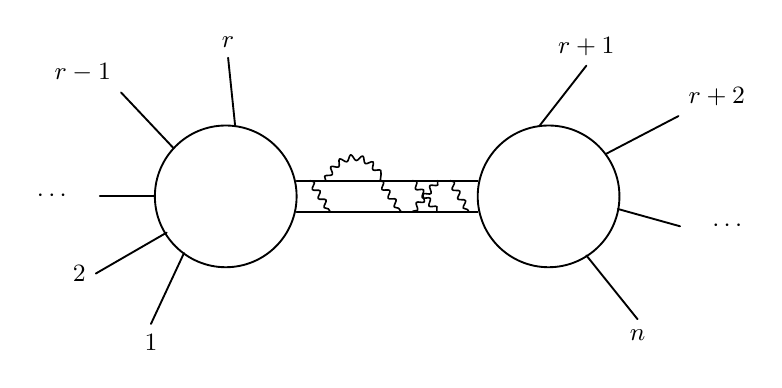
\begin{tikzpicture}[
  x=1cm,
  y=1cm,
  line cap=round,
  line join=round,
  line width=0.68pt,
  exchange/.style={
    line width=0.58pt,
    decorate,
    decoration={snake,amplitude=1.05pt,segment length=3.9pt}
  },
  every node/.style={font=\small}
]
  % The same arbitrary external subdiagrams as in Figure 10.2.
  \draw (-2.05,0) circle[x radius=0.90cm,y radius=0.90cm];
  \draw ( 2.05,0) circle[x radius=0.90cm,y radius=0.90cm];

  \draw (-2.58,-0.72) -- (-3.00,-1.62);
  \node[below] at (-3.00,-1.62) {$1$};
  \draw (-2.80,-0.46) -- (-3.70,-0.98);
  \node[left] at (-3.70,-0.98) {$2$};
  \draw (-2.95,0) -- (-3.65,0);
  \node[left] at (-3.94,0) {$\cdots$};
  \draw (-2.72,0.62) -- (-3.38,1.32);
  \node[above left] at (-3.38,1.32) {$r-1$};
  \draw (-1.93,0.89) -- (-2.02,1.76);
  \node[above] at (-2.02,1.76) {$r$};

  \draw (1.93,0.89) -- (2.53,1.66);
  \node[above] at (2.53,1.66) {$r+1$};
  \draw (2.78,0.54) -- (3.70,1.02);
  \node[above right] at (3.70,1.02) {$r+2$};
  \draw (2.93,-0.16) -- (3.72,-0.38);
  \node[right] at (4.00,-0.38) {$\cdots$};
  \draw (2.53,-0.75) -- (3.18,-1.56);
  \node[below] at (3.18,-1.56) {$n$};

  % Two elementary constituents propagating between the subdiagrams.
  \draw (-1.15,0.20) -- (1.15,0.20);
  \draw (-1.15,-0.20) -- (1.15,-0.20);

  % Representative exchanged particles in the infinite diagram class.
  \draw[exchange] (-0.98,0.20) -- (-0.72,-0.20);
  \draw[exchange] (-0.78,0.20)
    .. controls (-0.61,0.55) and (-0.26,0.55) .. (-0.08,0.20);
  \draw[exchange] (-0.10,0.20) -- (0.18,-0.20);
  \draw[exchange] (0.32,0.20) -- (0.64,-0.20);
  \draw[exchange] (0.64,0.20) -- (0.32,-0.20);
  \draw[exchange] (0.80,0.20) -- (1.04,-0.20);
\end{tikzpicture}
\caption{A Feynman diagram of the class whose sum has the pole structure
\eqref{eq:10.2.6}. Here the pole is due to a composite particle, a bound state
of two elementary particles. The elementary particles are represented by
straight lines, and interact by the exchange of particles represented by wavy
lines.}
\label{fig:10.3}
\end{figure}
\endgroup
